\documentclass[a4paper,10pt]{article}
\usepackage[utf8]{inputenc}

\title{Documentation for Half-Cheetah Control/Planning Using Mixed-Integer Optimization}
\author{Jiayi Wang}
\setlength{\parindent}{2em}
%\textwidth=15cm
\usepackage{indentfirst}

\addtolength{\oddsidemargin}{-.875in} %-.875
\addtolength{\evensidemargin}{-.875in}%-.875
\addtolength{\textwidth}{1.75in}%1.75

\addtolength{\topmargin}{-.875in}
\addtolength{\textheight}{1.75in}

\usepackage{graphicx}
\graphicspath{ {figures/} }

\PassOptionsToPackage{fleqn}{amsmath}		% math environments and more by the AMS 
\usepackage{amsmath}

\begin{document}

\maketitle

\section{Optimization Problem Formulation}

\subsection{Variables Definitions}

\begin{figure}[h!]
	\centering
	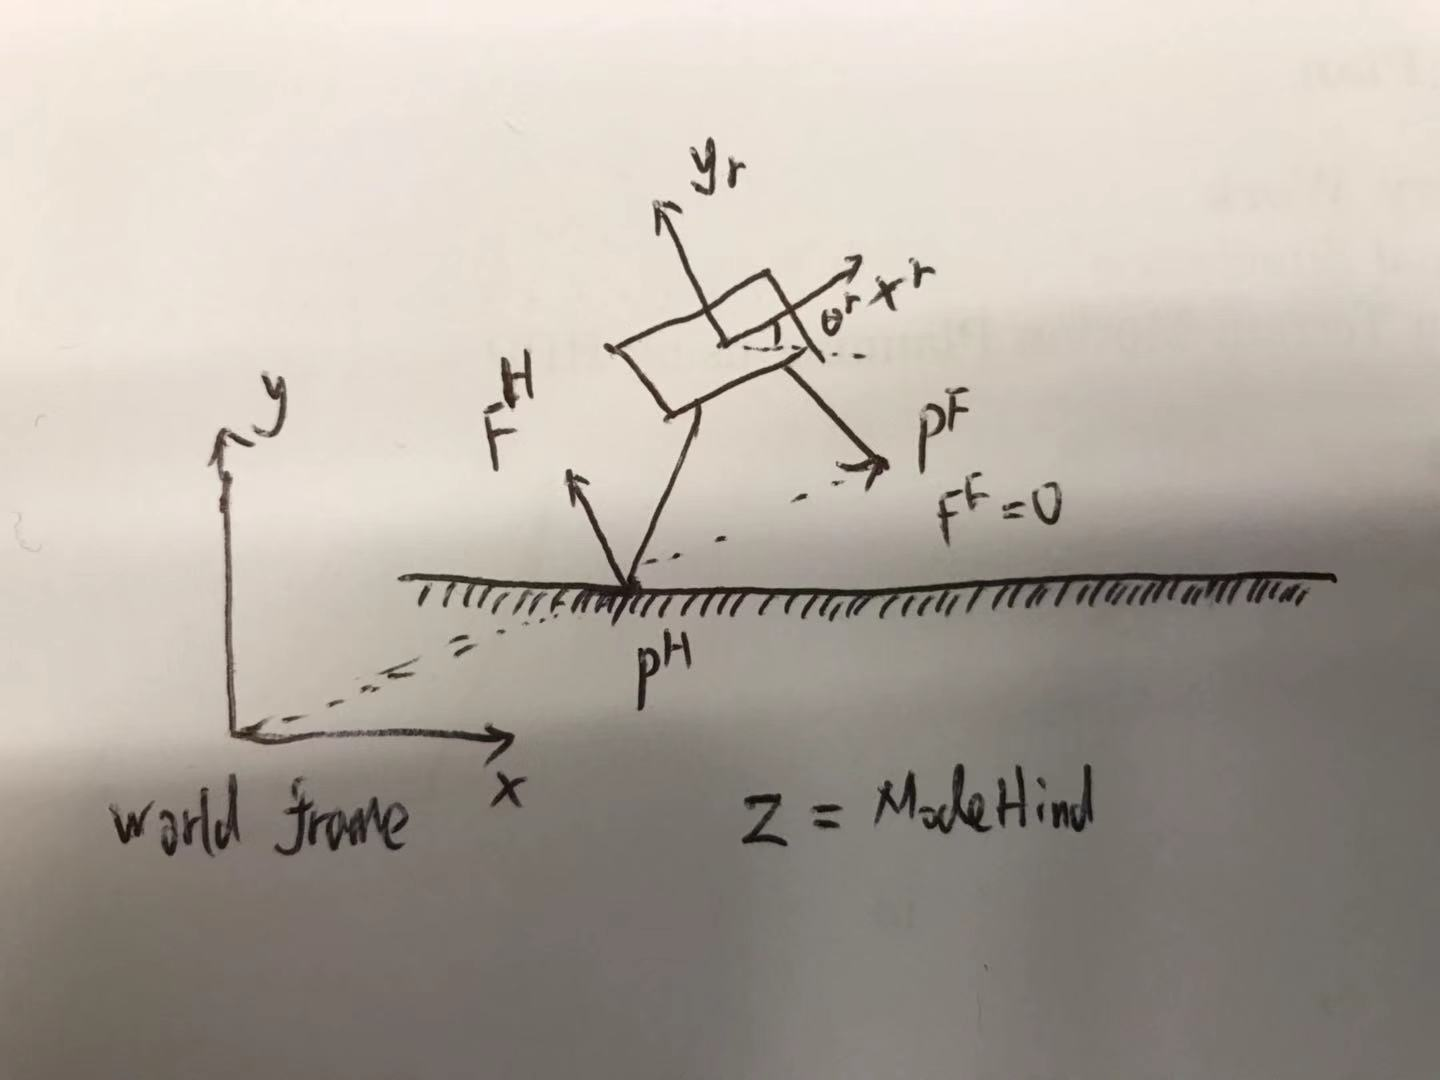
\includegraphics[scale = 0.3]{variable_definitions}
	\caption{Variable Definition for the 2D Half Cheetah Robot}
	\label{fig:variable_definitions}
\end{figure}

\textbf{Variables:}
\vspace{2mm}

Robot State: $ [x, y, \theta, \dot{x} ,\dot{y}, \dot{\theta}]$

$x$: Horizontal position of the torso

$y$: Vertical position of the torso

$\theta$: Torso orientation

$\dot{x}$: Horizontal Velocity of the torso

$\dot{y}$: Vertical Velocity of the torso

$\dot{\theta}$: Angular Velocity of the torso

\textbf{Define} $r = [x, y]$
\vspace{2mm}

\textbf{Foot/End-effector States (IN WORLD FRAME)}: 

\textbf{FrontLeg: }

Position: $P^F=[P^F_x,P^F_y]$

Velocity: $\dot{P}^F = [\dot{P}^F_x,\dot{P}^F_y]$

\vspace{2mm}

\textbf{HindLeg: }

Position: $P^H=[P^H_x, P^H_y]$

Velocity: $\dot{P}^H = [\dot{P}^H_x,\dot{P}^H_y]$
\vspace{2mm}

where $P^i_x$ and $P^i_y$ are the positions of $i^{th}$ foot/end-effector in \textbf{in world frame}, $i \in F, H$.
$\dot{P}^i_x$ and $\dot{P}^i_y$ are the velocities of $i^{th}$ foot/end-effector in \textbf{world frame}, $i \in F, H$.

\vspace{3mm}

\textbf{Foot-Ground Reaction Forces (IN WORLD FRAME)}:

FrontLeg: $F^F=[F^F_x,F^F_y]$

HindLeg: $F^H=[F^H_x,F^H_y]$
\vspace{2mm}

\textbf{Contact Modes (Discrete Variables; Two Tracks):}

\begin{itemize}
	\item \textbf{(Use only when necessary)} Mode Enumeration: $Mode = [Mode^{fly},Mode^{double},Mode^{front},Mode^{hind}]$, where $Mode^{name} = 0,1$
	
	\item \textbf{(Preferred)} Define Contact Configurations for Every Foot: $C = [C^F, C^H]$, where $C^i = 0,1$
	
	Using this formulation, we can keep dynamic constraints invariant, and ask all foot to obey complementarity constraints, kinematics constraint and friction cone. So, the foot-ground reaction forces may flow into system dynamics equation with zero values when legs are set as swing legs, or they will flow with some values to drive the torso to move, when they are set as stance legs.
	
	In contrary, the Mode Enumeration is tedious because we need to write different system dynamic constraint, footstep location, foot-ground reaction forces constraints (big-M) based on mode indicator variables.
	
\end{itemize}

\subsection{Objective/Cost Function}

\textbf{NOTE: For higher order integration scheme, we need to approximate the cost function using quadrature methods}

\textbf{Quadratic form:} $obj = v^TQv$

where $v$ is the decision variable vector, it should be a column vector, $Q$ is the selection matrix for the Quadratic Form.

\vspace{2mm}
$v^TQv = v_1Q_{11}v_1 + v_1Q_{12}v_2 + ... + v_2Q_{21}v_1 + v_2Q_{22}v_2 + ...$

$Q_{i,j} \in R^{dim(v_i) \times dim(v_j)}$ %make better

\subsection{Constraints}

\subsubsection{System Dynamics Constraint}

\textbf{System Dynamical Equations:}

\textbf{x-axis:}

$m\ddot{x} = F^F_x + F^H_x \rightarrow$

$\ddot{x} = \frac{F^F_x}{m} + \frac{F^H_x}{m} \rightarrow$

$\ddot{x} = f_x()$

\vspace{2mm}

\textbf{y-axis:}

$m\ddot{y} = -mg + F^F_y + F^H_y \rightarrow$

$\ddot{y} = -g + \frac{F^F_y}{m} + \frac{F^H_y}{m} \rightarrow$

$\ddot{y} = f_y()$
\vspace{2mm}

\textbf{rotation-axis:}

$I\ddot{\theta} = (P^F-r) \times F^F + (P^H -r) \times F^H \rightarrow$

$I\ddot{\theta} - (P^F-r) \times F^F - (P^H -r) \times F^H = 0$

\vspace{10mm}

\textbf{Quadrature Schemes:}

\textbf{Euler Integration (Currently in Use ):}

$x_{k+1}-x_k =h_kf_k \rightarrow$

$x_{k+1}-x_k-h_kf_k = 0$

\vspace{2mm}

\textbf{Trapezoidal Collocation:}

$x_{k+1}-x_k = \frac{1}{2}h_k(f_{k+1}+f_k) \rightarrow$

$x_{k+1}-x_k-\frac{1}{2}h_kf_{k+1}-\frac{1}{2}h_kf_k = 0$

\vspace{10mm}

\textbf{Apply Euler Integration into Dynamical Equations:}

\textbf{x-axis position (linear constraints; first-order):}

$x_{k+1} - x_k = h\dot{x_k} \rightarrow$

$x_{k+1} - x_k - h\dot{x_k} = 0$

\textbf{x-axis velocity (linear constraints; second-order):}

$\dot{x}_{k+1} - \dot{x}_k = \frac{h}{m}F^F_x + \frac{h}{m}F^H_x \rightarrow$

$\dot{x}_{k+1} - \dot{x}_k - \frac{h}{m}F^F_x - \frac{h}{m}F^H_x = 0$

\textbf{y-axis position (linear constraints; first-order):}

$y_{k+1} - y_k = h\dot{y}_k \rightarrow$

$y_{k+1} - y_k - h\dot{y}_k = 0$

\textbf{y-axis velocity (linear constraints; second-order):}

$\dot{y}_{k+1} - \dot{y}_k = -hg + \frac{h}{m}F^F_y + \frac{h}{m}F^H_y \rightarrow$

$\dot{y}_{k+1} - \dot{y}_k - h\frac{F^F_y}{m} - h\frac{F^H_y}{m} = -hg$

\textbf{rotation-axis position (linear constraints; first-order):}

$\theta_{k+1} - \theta_k = h\dot{\theta} \rightarrow$

$\theta_{k+1} - \theta_k - h\dot{\theta} = 0$

\vspace{3mm}

\textbf{rotation-axis velocity Vector Form  (Nonlinear Constraints; second order):}

$I\dot{\theta}_{k+1} - I\dot{\theta}_k = h[(P^F_k - r_k) \times F^F_k + (P^H_k - r_k) \times F^H_k] \rightarrow$

$I\dot{\theta}_{k+1} - I\dot{\theta}_k - h[(P^F_k - r_k) \times F^F_k - (P^H_k - r_k) \times F^H_k = 0$

\textbf{Cross Product Note: }

$a = [a_x, a_y], b = [b_x, b_y]$

$a \times b = a_xb_y - a_yb_x$

\textbf{Cross Produce of Contact Forces and Foot Position Vectors:}

$\tau^{sum}_k = (P^F_{x,k} - x_k)F^F_{y,k} - (P^F_{y,k} - y_k)F^F_{x,k} + (P^H_{x,k} - x_k)F^H_{y,k} - (P^H_{y,k} - y_k)F^H_{x,k} $

\textbf{Then rotation axis velocity contraints becomes (Nonlinear Constraints; second order):}

$I\dot{\theta}_{k+1} - I\dot{\theta}_k - h\tau^{sum}_k = 0 \rightarrow$

$I\dot{\theta}_{k+1} - I\dot{\theta}_k - h[(P^F_{x,k} - x_k)F^F_{y,k} - (P^F_{y,k} - y_k)F^F_{x,k} + (P^H_{x,k} - x_k)F^H_{y,k} - (P^H_{y,k} - y_k)F^H_{x,k}] = 0$

\vspace{10mm}

\textbf{Apply Trapezoidal Collocation into Dynamical Equations (Currently Not in Use; Missing Rotation Dynamics):}

\textbf{x-axis position (linear constraints; first-order):} 

$x_{k+1}-x_k=\frac{1}{2}h_k(\dot{x}_{k+1}+\dot{x}_k) \rightarrow$

$x_{k+1}-x_k-\frac{1}{2}h_k\dot{x}_{k+1}-\frac{1}{2}h_k\dot{x}_k = 0$

\textbf{x-axis velocity (linear constraints; second-order): }

$\dot{x}_{k+1}-\dot{x}_k-\frac{1}{2}h_k(\frac{F^F_{x,k+1}}{m}+\frac{F^H_{x,k+1}}{m})-\frac{1}{2}h_k(\frac{F^F_{x,k}}{m}+\frac{F^H_{x,k}}{m}) = 0 \rightarrow$

$\dot{x}_{k+1}-\dot{x}_k-\frac{1}{2}h_k\frac{F^F_{x,k+1}}{m}-\frac{1}{2}h_k\frac{F^H_{x,k+1}}{m}-\frac{1}{2}h_k\frac{F^F_{x,k}}{m}-\frac{1}{2}h_k\frac{F^H_{x,k}}{m} = 0$

\textbf{y-axis position (linear constraints; first-order):} 

$y_{k+1}-y_k = \frac{1}{2}h_k(\dot{y}_{k+1}+\dot{y}_k) \rightarrow$

$y_{k+1}-y_k-\frac{1}{2}h_k\dot{y}_{k+1}-\frac{1}{2}h_k\dot{y}_k = 0$

\textbf{y-axis velocity (linear constraints; second-order):}

$\dot{y}_{k+1}-\dot{y}_k-\frac{1}{2}h_k(-g+\frac{F^F_{y,k+1}}{m}+\frac{F^H_{y,k+1}}{m})-\frac{1}{2}h_k(-g+\frac{F^F_{y,k}}{m}+\frac{F^H_{y,k}}{m}) = 0 \rightarrow $

$\dot{y}_{k+1}-\dot{y}_k + \frac{1}{2}h_kg - \frac{1}{2}h_k\frac{F^F_{y,k+1}}{m} - \frac{1}{2}h_k\frac{F^H_{y,k+1}}{m} + \frac{1}{2}h_kg - \frac{1}{2}h_k\frac{F^F_{y,k}}{m} - \frac{1}{2}h_k\frac{F^H_{y,k}}{m} = 0 \rightarrow$

$\dot{y}_{k+1}-\dot{y}_k  - \frac{1}{2}h_k\frac{F^F_{y,k+1}}{m} - \frac{1}{2}h_k\frac{F^H_{y,k+1}}{m}  - \frac{1}{2}h_k\frac{F^F_{y,k}}{m} - \frac{1}{2}h_k\frac{F^H_{y,k}}{m} = - h_kg$

\vspace{10mm}

\textbf{Foot/End-effector Dynamics:}

\vspace{2mm}

\textbf{Euler Integration Formulation: }

\textbf{Front Leg x-axis position (linear constraint; first-order): }

$P^F_{x,k+1} - P^F_{x,k} = h\dot{P}^F_{x,k} \rightarrow$

$P^F_{x,k+1} - P^F_{x,k} - h\dot{P}^F_{x,k} = 0$

\textbf{Front Leg y-aixs position (linear constraint; first-order): }

$P^F_{y,k+1} - P^F_{y,k} = h\dot{P}^F{y,k} \rightarrow$

$P^F_{y,k+1} - P^F_{y,k} - h\dot{P}^F_{y,k} = 0 $

\textbf{Hind Leg x-axis position (linear constraint; first-order):}

$P^H_{x,k+1} - P^H_{x,k} = h\dot{P}^H_{x,k} \rightarrow$

$P^H_{x,k+1} - P^H_{x,k} - h\dot{P}^H_{x,k} = 0$

\textbf{Hind Leg y-axis position (linear constraint; first order): }

$P^H_{y,k+1} - P^H_{y,k} = h\dot{P}^H_{y,k}$

$P^H_{y,k+1} - P^H_{y,k} - h\dot{P}^H_{y,k} = 0$

\vspace{5mm}

\textbf{Trapezoidal Quadrature for Foot Dynamics (Not in Use, because it cannot handle the discontinuity of control signals, introduced by contact mode switches)]}

Front Leg:

FrontLeg x-axis: 

$P^F_{x,k+1}-P^F_{x,k} = \frac{1}{2}h_k(\dot{P}^F_{x,k+1}+\dot{P}^F_{x,k}) \rightarrow P^F_{x,k+1}-P^F_{x,k} - \frac{1}{2}h_k\dot{P}^F_{x,k+1} - \frac{1}{2}h_k\dot{P}^F_{x,k}  = 0$

\vspace{2mm}

FrontLeg y-axis:

$P^F_{y,k+1}-P^F_{y,k} = \frac{1}{2}h_k(\dot{P}^F_{y,k+1}+\dot{P}^F_{y,k}) \rightarrow P^F_{y,k+1}-P^F_{y,k} - \frac{1}{2}h_k\dot{P}^F_{y,k+1} - \frac{1}{2}h_k\dot{P}^F_{y,k}  = 0$

\vspace{3mm}

Hind Leg:

HindLeg x-axis:

$P^H_{x,k+1}-P^H_{x,k} = \frac{1}{2}h_k(\dot{P}^H_{x,k+1}+\dot{P}^H_{x,k}) \rightarrow P^H_{x,k+1}-P^H_{x,k} - \frac{1}{2}h_k\dot{P}^H_{x,k+1} - \frac{1}{2}h_k\dot{P}^H_{x,k}  = 0$

\vspace{2mm}

HindLeg y-axis:

$P^H_{y,k+1}-P^H_{y,k} = \frac{1}{2}h_k(\dot{P}^H_{y,k+1}+\dot{P}^H_{y,k}) \rightarrow P^H_{y,k+1}-P^H_{y,k} - \frac{1}{2}h_k\dot{P}^H_{y,k+1} - \frac{1}{2}h_k\dot{P}^H_{y,k}  = 0$

\vspace{3mm}

\subsubsection{Complementarity Constraint:}
\vspace{2mm}

\textbf{General Idea:}

\begin{itemize}
	\item if $C^i = 1 \rightarrow $ foot in contact, then
		
		\begin{itemize}
			\item Foot stay on the ground: $P_y = 0$ or $P_y = height(P_x,Py)$ (terrain height map)
			\item Vertical force pointing upwards: $F_y \geq 0$
			\item Non-slippage: $\dot{P}_x = 0, \dot{P}_y =0$ (may remove if we want slippage dynamics in the future) (SEE if there are other better way to define end-effector velocity, using footstep locations only)
			
			May use logical variables, $z_{k+1}$ and $z_{k} = 0/1?$ to identify phase boundaries and knots inside a phase.
		\end{itemize}
	
	\item if $C^i =0 \rightarrow $ foot in the air, then
	
		\begin{itemize}
			\item No forces: $F_x = 0, F_y =0$
			\item Foot above the terrain: $P_y \geq 0$
		\end{itemize}
\end{itemize}

\vspace{3mm}

\textbf{In Optimizer Constraint Form:}

\begin{itemize}
	\item Foot/End-effector position:
	
	$P_y \leq height + M^{pos}(1-C)$
	
	$P_y \geq height$
	
	\item Foot/End-Effector Velocity:
	
	x-axis:
	
	$\dot{P}_x \leq 0 + M^{vel}(1-C)$
	
	$\dot{P}_x \geq 0 - M^{vel}(1-C)$
	
	y-axis:
	
	$\dot{P}_y \leq 0 + M^{vel}(1-C)$
	
	$\dot{P}_y \geq 0 - M^{vel}(1-C)$
	
	\item Foot-ground reaction forces:
	
	x-axis:
	
	$F_x \leq 0 + M^fC$
	
	$F_x \geq 0 - M^fC$
	
	y-axis:
	
	$F_y \leq 0 + M^fC$
	
	$F_y \geq 0$
	
\end{itemize}

\vspace{3mm}

\textbf{Complete form for Programming:}

\textbf{Front Leg:}

\begin{itemize}
	\item Foot/End-Effector Position (y-axis only):
	
	$P^F_y \leq height + M^{pos}_y(1-C^F) \rightarrow P^F_y +  M^{pos}_yC^F \leq height + M^{pos}_y$
	
	\vspace{2mm}
	
	$P^F_y \geq height$
	
	\item Foot/End-effector Velocity:
	
	x-axis:
	
	$\dot{P}^F_x \leq 0 + M^{vel}(1-C^F) \rightarrow \dot{P}^F_x + M^{vel}C^F \leq 0 + M^{vel}$
	
	$\dot{P}^F_x \geq 0 - M^{vel}(1-C^F) \rightarrow \dot{P}^F_x - M^{vel}C^F \geq 0 - M^{vel}$
	
	y-axis:
	
	$\dot{P}^F_y \leq 0 + M^{vel}(1-C^F) \rightarrow \dot{P}^F_y + M^{vel}C^F \leq 0 + M^{vel}$
	
	$\dot{P}^F_y \geq 0 - M^{vel}(1-C^F) \rightarrow \dot{P}^F_y - M^{vel}C^F \geq 0 - M^{vel}$
	
	\item Foot-Ground Reaction Forces:
	
	x-axis:
	
	$F^F_x \leq 0 + M_{fx}C^F \rightarrow F^F_x - M^fC^F \leq 0$
	
	$F^F_x \geq 0 - M_{fx}C^F \rightarrow F^F_x + M^fC^F \geq 0$
	
	y-axis:
	
	$F^F_y \leq 0 + M_{fy}C^F \rightarrow F^F_y - M^fC^F \leq 0$
	
	$F^F_y \geq 0$
	
\end{itemize}

\textbf{Hind Leg:}

\begin{itemize}
	\item Foot/End-Effector Position:
	
	$P^H_y \leq height + M^{pos}_y(1-C^H) \rightarrow P^H_y +  M^{pos}_yC^H \leq height + M^{pos}_y$
	
	$P^H_y \geq height$
	
	\item Foot/End-effector Velocity:
	
	x-axis:
	
	$\dot{P}^H_x \leq 0 + M^{vel}(1-C^H) \rightarrow \dot{P}^H_x + M^{vel}C^H \leq 0 + M^{vel}$
	
	$\dot{P}^H_x \geq 0 - M^{vel}(1-C^H) \rightarrow \dot{P}^H_x - M^{vel}C^H \geq 0 - M^{vel}$
	
	y-axis:
	
	$\dot{P}^H_y \leq 0 + M^{vel}(1-C^H) \rightarrow \dot{P}^H_y + M^{vel}C^H \leq 0 + M^{vel}$
	
	$\dot{P}^H_y \geq 0 - M^{vel}(1-C^H) \rightarrow \dot{P}^H_y - M^{vel}C^H \geq 0 - M^{vel}$
	
	\item Foot-Ground Reaction Forces:
	
	x-axis:
	
	$F^H_x \leq 0 + M^fC^H \rightarrow F^H_x - M^fC^H \leq 0$
	
	$F^H_x \geq 0 - M^fC^H \rightarrow F^H_x + M^fC^H \geq 0$
	
	y-axis:
	
	$F^H_y \leq 0 + M^fC^H \rightarrow F^H_y - M^fC^H \leq 0$
	
	$F^H_y \geq 0$
	
\end{itemize}

\vspace{3mm}

\subsubsection{Kinematics Constraint (Nonlinear Constraints)}

\begin{figure}[h!]
	\centering
	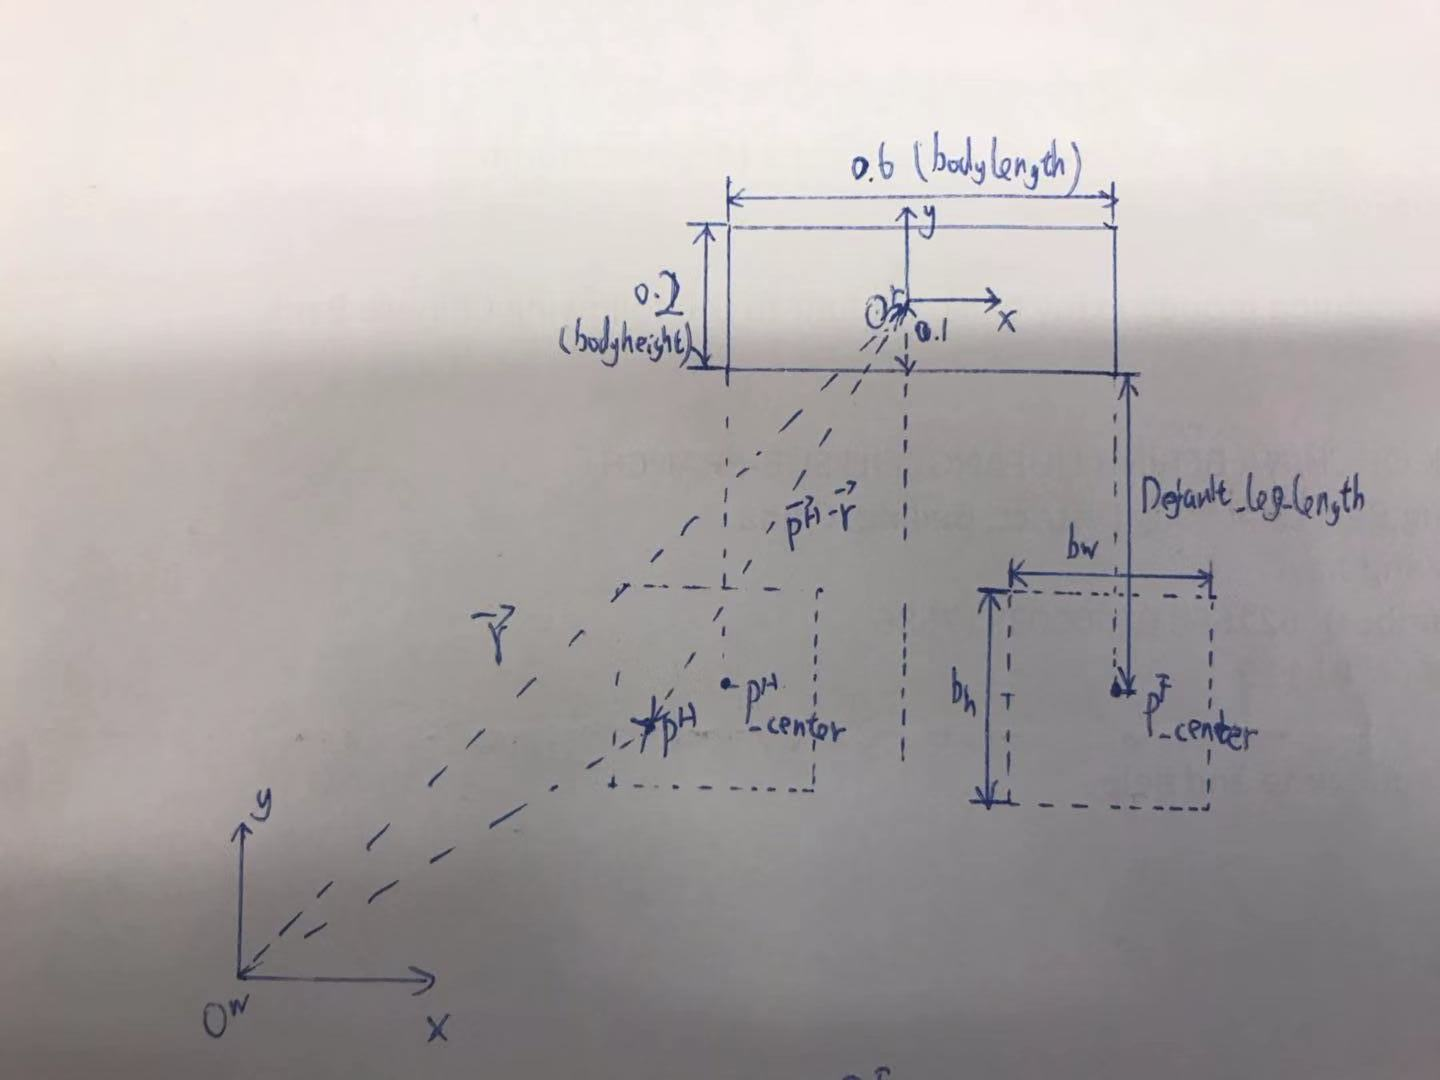
\includegraphics[scale = 0.3]{KinematicsConstraint}
	\caption{Kinematics Constraint of the 2D Half Cheetah Robot}
	\label{fig:kinematics_contraint}
\end{figure}

\textbf{Variable Definitions:}

Body Length: $L_{Body}$

Body Height: $H_{Body}$

Default Leg Length: $\bar{L}_{leg}$

Default (Center) Position of Front Leg (\textbf{in robot local frame}): 

$P^F_{center} = [\frac{1}{2}L_{Body}, -(\frac{1}{2}H_{Body} + \bar{L}_{leg})] $

Default (Center) Position of Hind Leg (\textbf{in robot local frame}): 

$P^H_{center} = [-\frac{1}{2}L_{Body}, -\frac{1}{2}H_{Body} + \bar{L}_{leg}]$

Width of the bounding box: $b_w$

Height of the bounding box: $b_h$

bounding box vector: $b = [b_w, b_h]$

\vspace{3mm}

\textbf{Kinematics Constraint (Augment to be consistent with program):}

$-b/2 \leq R(\theta_k)(P_k-r_k) - P_{center} \leq b/2$

\vspace{3mm}

\subsubsection{Friction Cone Constraint (Nonlinear Constraint for Uneven Terrain)}

\textbf{Variable Definition:}

Terrain Norm: $N = [N_x, N_y]$

Terrain Norm will become a function of $r = [x,y]$ for uneven terrain cases

Friction Coefficient: $\mu$

\vspace{3mm}

Friction Cone Constraint:

In 2D:

$F^F_{x,k} \leq \mu(N_x(r_k)F_{x,k} + N_y(r_k)F_{y,k})$

In 3D \textbf{(Nonlinear Constraint):}

$\sqrt{F^2_x + F^2_y} \leq \mu f_n$

$f_n = [F^F_x,F^F_y]'*[N_x,N_y]$



\subsubsection{Boundary Constraints}

Initial Condition: 

$x_0 = x(0)$

$y_0 = y(0)$

$\theta_0 = \theta(0)$

$\dot{x}_0 = \dot{x}(0)$

$\dot{y}_0 = \dot{y}(0)$

$\dot{\theta}_0 = \dot{\theta}(0)$

\vspace{2mm}

Terminal Condition:

$x_T = x(T)$

$y_T = y(T)$

$\theta_T = \theta(T)$

$\dot{x}_T = \dot{x}(T)$

$\dot{y}_T = \dot{y}(T)$

$\dot{\theta}_T = \dot{\theta}(T)$

\vspace{3mm}

\subsubsection{Switching Time}

Introduce a variable $\tau \in [0,1]$, the upper bound of $\tau$ can be larger but better take it normalised.

Cut $\tau$ into N phases.

Switching Time Vector (Terminal Time of Each Phase)
$Ts = [Ts_1, Ts_2, ... , Tend]$

Integration Step for each Phase:

$h = N*(Ts_{i+1}-Ts_{i})*\tau_h$

Switching Time Follow the Constraint:

(1) $0 \leq Ts_1 \leq Ts_2 ... \leq Tend$

where $\tau_h = $ 1/Number of Knots


\section{To-Do List}
\begin{enumerate}
	\item Add testing functions, checking by verifying matrix dimensionality.
	\item Foot/End-effector velocity constraint, is there any better to define it, to remove end-effector velocity state, using logical operations.
\end{enumerate}

\medskip
\newpage
\bibliographystyle{unsrt}%Used BibTeX style is unsrt
\bibliography{sample}

\end{document}
